\documentclass[a4paper, 11pt]{article}
\usepackage[utf8]{inputenc} % Change according your file encoding
\usepackage{float}
\usepackage{graphicx}
\usepackage{url}

%opening
\title{HW1 Report, Rudy: A Small Web Server}
\author{David Fischer}
\date{\today{}}

\begin{document}

\maketitle

\section{Introduction}

As part of this report a HTTP/1.1 server partially implementing the RFC 2616\footnote{\url{https://www.ietf.org/rfc/rfc2616.txt}} specification was created in the Erlang programming language.
The server is capable of correctly parsing and responding to HTTP requests, handling multiple clients concurrently, and acting as a file server with functional encoding. xxx todo how related to dist system, why important

\section{Main problems and solutions}

\subsection{Scope}

As the HTTP/1.1 specification is quite broad building up scope creep beyond the goals of the original assignment was a concern. Work was limited to objectives specifically mentioned in the assignment description.
At time of submission the server currently supports the following features:
\begin{itemize}
\item Listening on a specified port and delegating requests to one or many handler processes
\item Parsing HTTP $GET$ and $POST$ requests (URI, request headers, and body)
\item Responding with one of three HTTP status codes: $200$ OK, $404$ Not Found, or $500$ Internal Server Error
\item Serving static files from the working directory and its subdirectories with a limited number of supported media types
\item Support for the Accept-Enconding request header, specifically gzip
\end{itemize}

\subsection{Erlang}
todo
\section{Evaluation}

Testing the baseline implementation of \textit{Rudy}, including the artificial 40ms delay, with the given benchmark program measures 100 requests in 4.916 seconds, or $\approx$20 requests per second.
Since the benchmark runs sequentially, the regular parsing overhead can be calculated as 9,16 ms meaning the artificial delay is over four times the length of a regular request.

Additionally, while the artificial delay isn't noticeable with a single instance of the benchmark running, starting a second run from another machine doubles the request time while the benchmarks overlap as can be seen in Figure \ref{fig:results1}.

\begin{figure}[H]
  \begin{center}
    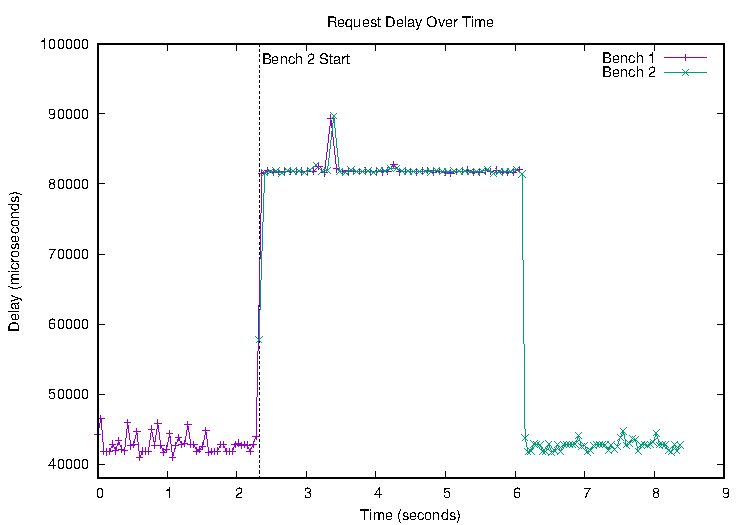
\includegraphics{graphs/requests-single-process/requests.pdf}
    \caption{Single Process Handler}
    \label{fig:results1}
  \end{center}
\end{figure}

This outcome is expected, as a single handler process will always be blocked while already responding to a request during which all new requests are waiting to be picked up.
To solve this and increase throughput, Erlangs support for having multiple processes listen to the same socket was utilized.
Figure \ref{fig:results2} shows the same two sequential benchmarks running against an instance of \textit{Rudy} with two handler processes running, resulting in no spike in response delay.

\begin{figure}[H]
  \begin{center}
    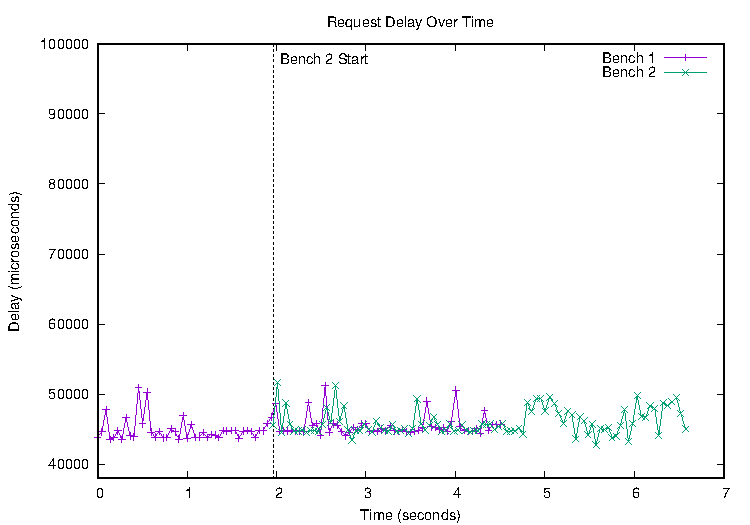
\includegraphics{graphs/requests-multi-process/requests.pdf}
    \caption{Multi-Process Handler}
    \label{fig:results2}
  \end{center}
\end{figure}

\subsection{File Server Functionality}
The implementation of \textit{Rudy} supports serving gzip compressed files including a limited selection of MIME types. xxx
\begin{figure}[H]
  \begin{center}
    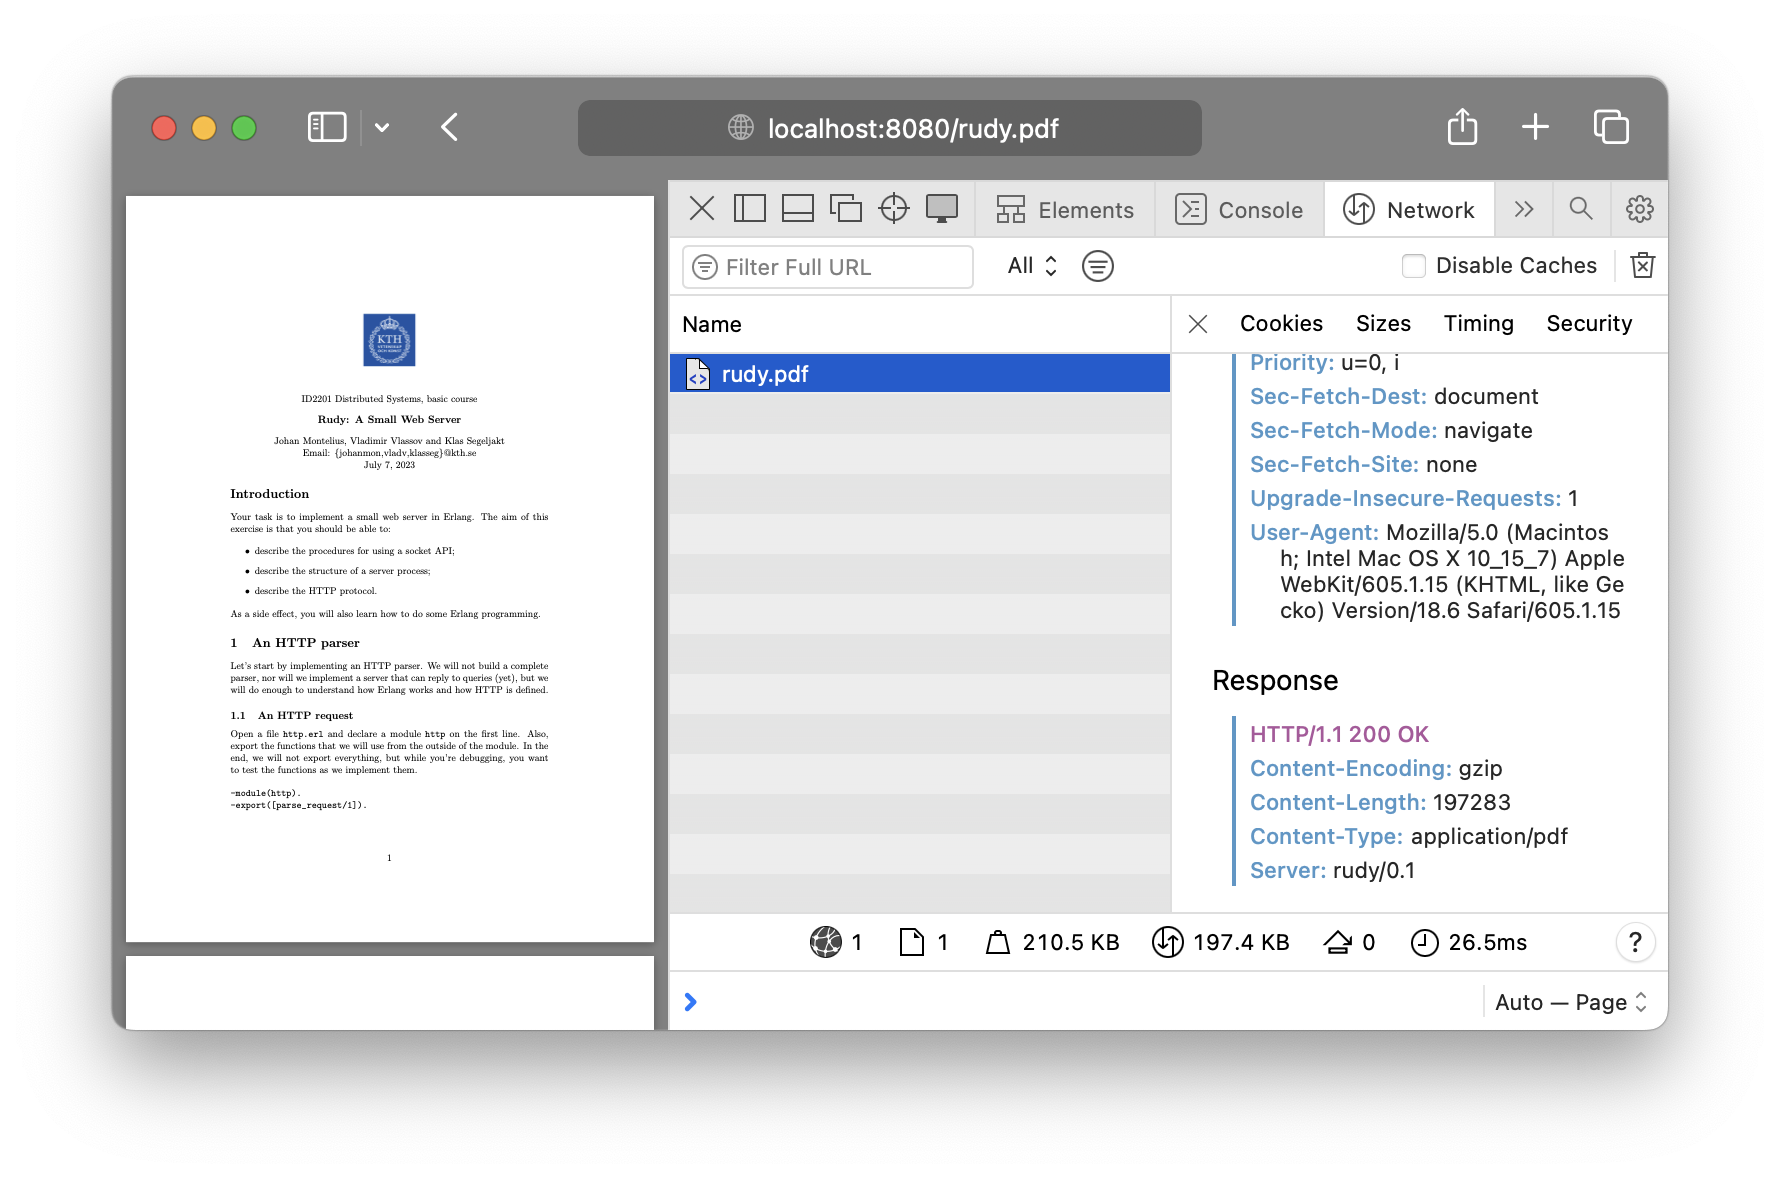
\includegraphics[height=200px]{graphs/browser/pdf-gzip.png}
    \caption{\textit{Rudy} serving a gzipped PDF file to a browser}
    \label{fig:browser1}
  \end{center}
\end{figure}

\begin{enumerate}
\item one
\item two
\end{enumerate}

\section{Conclusions}

xxx What have you learnt from the problem presented? Was it useful?


\end{document}
